\documentclass[mathNotesPreamble]{subfiles}
\begin{document}
%\relscale{1.4} %TODO
\section{16.3: Double Integrals in Polar Coordinates}

  Suppose we wish to find the volume bounded by the curve $f(x,y)=9-x^2-y^2$ and the $xy$-plane. The region of integration would be 
    \[R=\set{(x,y): -3\leq x\leq 3, -\sqrt{9-x^2}\leq y\leq \sqrt{9-x^2}}\]

    \noindent
    \begin{minipage}{0.5\linewidth}
      \[\int_{-3}^{3}\int_{-\sqrt{9-x^2}}^{\sqrt{9-x^2}} 9-x^2-y^2\,dy\,dx\]
    \end{minipage}%
    \begin{minipage}{0.5\linewidth}
      \begin{flushright}
        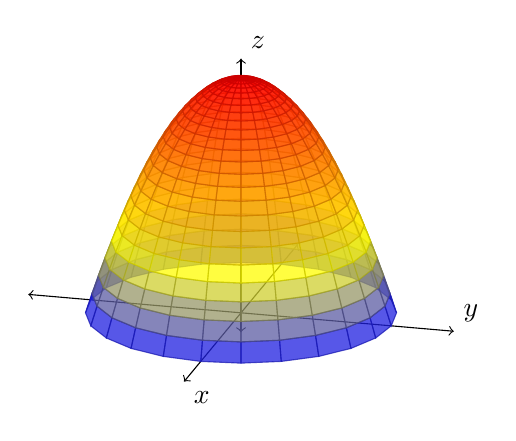
\begin{tikzpicture}
          \begin{axis}[
            axis lines=center,
            axis line style={black,<->},
            xmin=-3.5,  xmax=3.5,  xmajorticks=false,
            ymin=-3.5,  ymax=3.5,  ymajorticks=false,
            zmin=0,     zmax=9,  zmajorticks=false,
            enlargelimits={abs=0.75},
            ticklabel style={font=\normalsize,inner sep=0.5pt,fill=white,opacity=1.0, text opacity=1},
            xlabel=$x$, xlabel style={at={(ticklabel* cs:1)},anchor=north west},
            ylabel=$y$, ylabel style={at={(ticklabel* cs:1)},anchor=south west},
            zlabel=$z$, zlabel style={at={(ticklabel* cs:1)},anchor=south west},
            view={105}{27.5},
            ]
            \addplot3 [surf, draw=none, opacity=0.75, restrict z to domain=0:9, data cs=polar, domain=0:360, y domain=0:3] (x, y, 9-y^2);
          \end{axis}
        \end{tikzpicture}
      \end{flushright}
    \end{minipage}%
  \vspace*{\stretch{1}}

  \noindent
  Alternatively, we can use polar coordinates where $x=r\cos(\theta)$ and $y=r\sin(\theta)$. The associated region $R$ is called a \textbf{polar rectangle}.

  \begin{thmBox*}[Theorem 16.3: Change of Variables for Double Integrals over Polar Rectangle Regions]
    Let $f$ be continuous on the region $R$ in the $xy$-plane expressed in polar coordinates a s$R=\set{(r,\theta): 0\leq a\leq r\leq b, \alpha\leq\theta\leq \beta}$, where $\beta-\alpha=2\pi$. Then $f$ is integrable over $R$, and the double integral of $f$ over $R$ is
      \[\iint\limits_R f(x,y)\,dA=\int_\alpha^\beta \int_a^b f\parens{r\cos\theta,\, r\sin\theta}\,r\,dr\,d\theta.\]
  \end{thmBox*}
  \textit{Note:} When we convert to polar coordinates, there is an extra factor of $r$. This is due to the area of the circular segment being $\frac{1}{2}r^2\theta$ (Section 16.7 will elaborate on this).
  \pagebreak

  \begin{ex*}
    Graph the following regions:
  \end{ex*}
  \begin{tasks}[after-item-skip=\stretch{1},label=](1)
    \task 
      \begin{minipage}[t]{0.5\linewidth}\mbox{}
        $\displaystyle R=\set{(r,\theta): 0\leq r\leq1,\ 0\leq \theta\leq \frac{5\pi}{4}}$
      \end{minipage}%
      \begin{minipage}[t]{0.5\linewidth}\mbox{}
      \vspace*{-2\baselineskip}
        \begin{flushright}
          \begin{tikzpicture}
            \begin{axis}[
              grid=both, %major,minor
              grid style={line width=0.35pt, draw=gray!75},
              axis equal,
              axis lines=center,
              axis line style={black,->},
              xmin=-2.5, xmax=2.5,
              ymin=-2.25, ymax=2.25,
              ticklabel style={font=\footnotesize,inner sep=0.5pt,fill=white,
                opacity=1.0, text opacity=1},
              every axis plot/.append style={line width=0.95pt, color=blue, samples=100}
              ]
            \end{axis}
          \end{tikzpicture}
        \end{flushright}
      \end{minipage}
    \task 
      \begin{minipage}[t]{0.5\linewidth}\mbox{}
        $\displaystyle R=\set{(r,\theta): 2\leq r\leq 4,\ -\frac{\pi}{6}\leq \theta\leq \frac{7\pi}{6}}$
      \end{minipage}%
      \begin{minipage}[t]{0.5\linewidth}\mbox{}
      \vspace*{-2\baselineskip}
        \begin{flushright}
          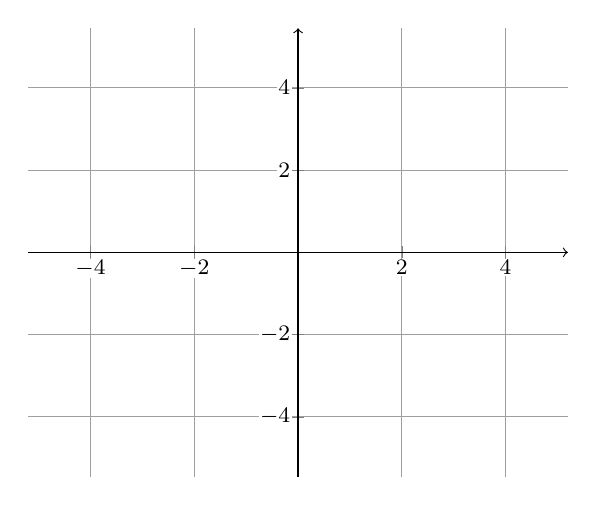
\begin{tikzpicture}
            \begin{axis}[
              grid=both, %major,minor
              grid style={line width=0.35pt, draw=gray!75},
              axis lines=center,
              axis line style={black,->},
              xmin=-4.25, xmax=4.25,
              ymin=-4.5,  ymax=4.5,
              enlargelimits={abs=0.95},
              ticklabel style={font=\footnotesize,inner sep=0.5pt,fill=white,
                opacity=1.0, text opacity=1},
              every axis plot/.append style={line width=0.95pt, color=blue, samples=100}
              ]
            \end{axis}
          \end{tikzpicture}
        \end{flushright}
      \end{minipage}
  \end{tasks}
  \vspace*{\stretch{1}}
  \pagebreak

  \begin{ex*}
    Consider the paraboloid given earlier: Find the volume of the solid bounded above by $z=9-x^2-y^2$ and below by the $xy$-plane.
  \end{ex*}
  \vspace{\stretch{1}}
  \begin{flushright}
    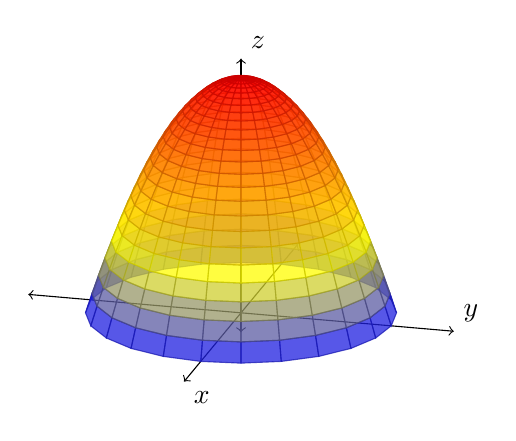
\begin{tikzpicture}
      \begin{axis}[
        axis lines=center,
        axis line style={black,<->},
        xmin=-3.5,  xmax=3.5,  xmajorticks=false,
        ymin=-3.5,  ymax=3.5,  ymajorticks=false,
        zmin=0,     zmax=9,  zmajorticks=false,
        enlargelimits={abs=0.75},
        ticklabel style={font=\normalsize,inner sep=0.5pt,fill=white,opacity=1.0, text opacity=1},
        xlabel=$x$, xlabel style={at={(ticklabel* cs:1)},anchor=north west},
        ylabel=$y$, ylabel style={at={(ticklabel* cs:1)},anchor=south west},
        zlabel=$z$, zlabel style={at={(ticklabel* cs:1)},anchor=south west},
        view={105}{27.5},
        ]
        \addplot3 [surf, draw=none, opacity=0.75, restrict z to domain=0:9, data cs=polar, domain=0:360, y domain=0:3] (x, y, 9-y^2);
      \end{axis}
    \end{tikzpicture}
  \end{flushright}
  \pagebreak

  \begin{ex*}
    Find the area of the solid bounded below by the paraboloid $z=x^2+y^2$ and bounded above by the cone $z=2-\sqrt{x^2+y^2}$.
  \end{ex*}
  \vspace{\stretch{1}}
  \begin{flushright}
    \begin{tikzpicture}
      \begin{axis}[
        axis lines=center,
        axis line style={black,<->},
        xmin=-1.05,  xmax=1.05,  xmajorticks=false,
        ymin=-1.05,  ymax=1.05,  ymajorticks=false,
        zmin=0,      zmax=2.15,  zmajorticks=false,
        ticklabel style={font=\normalsize,inner sep=0.5pt,fill=white,opacity=1.0, text opacity=1},
        xlabel=$x$, xlabel style={at={(ticklabel* cs:1)},anchor=north west},
        ylabel=$y$, ylabel style={at={(ticklabel* cs:1)},anchor=south west},
        zlabel=$z$, zlabel style={at={(ticklabel* cs:1)},anchor=south west},
        view={105}{27.5},
        ]
        \addplot3 [surf, draw=none, opacity=0.5, restrict z to domain=0:2, data cs=polar, domain=0:360, y domain=0:1] (x, y, y^2);
        \addplot3[domain=0:2*pi, samples=100, samples y=0, -, ClemsonPurple, line width=1pt] ({cos(deg(x))},{sin(deg(x))},1);
        \addplot3 [surf, draw=none, opacity=0.5, restrict z to domain=0:2, data cs=polar, domain=0:360, y domain=0:1] (x, y, 2-y);
      \end{axis}
    \end{tikzpicture}
  \end{flushright}
  \pagebreak

  \begin{ex*}
    Find the volume of the region beneath the surface $z=xy+10$ and above the annular region $R=\set{(r,\theta): 2\leq r\leq 4,\ 0\leq \theta\leq 2\pi}$.
  \end{ex*}
  \vspace*{\stretch{1}}
  \begin{flushright}
    \begin{tikzpicture}
      \begin{axis}[
        axis lines=center,
        axis line style={black,->},
        xmin=-4.5,   xmax=4.5,  xmajorticks=false,
        ymin=-4.5,   ymax=4.5,  ymajorticks=false,
        zmin=0,      zmax=16,   zmajorticks=false,
        ticklabel style={font=\normalsize,inner sep=0.5pt,fill=white,opacity=1.0, text opacity=1},
        view={110}{35},
        ]
        \addplot3[name path =A, domain=0:2*pi, samples=100, samples y=0, -, ClemsonPurple, line width=1pt] ({2*cos(deg(x))},{2*sin(deg(x))},0);
        \addplot3[name path =B, domain=0:2*pi, samples=100, samples y=0, -, ClemsonPurple, line width=1pt] ({4*cos(deg(x))},{4*sin(deg(x))},0);
        \addplot3 [ClemsonPurple!50, opacity=0.5] fill between [of=A and B];
        \addplot3 [surf, draw=none, opacity=0.95, restrict z to domain=0:26, data cs=polar, samples=20, domain=-180:0, y domain=2:4] (x, y, {10+y^2*cos(x)*sin(x)});
        \addplot3 [surf, draw=none, opacity=0.95, restrict z to domain=0:26, data cs=polar, samples=20, domain=130:310, y domain=2:4] (x, y, {10+y^2*cos(x)*sin(x)});
        \addplot3 [surf, draw=none, opacity=0.95, restrict z to domain=0:26, data cs=polar, samples=20, domain=-50:130, y domain=2:4] (x, y, {10+y^2*cos(x)*sin(x)});
      \end{axis} 
    \end{tikzpicture}
  \end{flushright}
  \pagebreak 

  \vspace*{\stretch{1}}
  \begin{thmBox*}[Theorem 16.4: Change of Variables for Double Integrals over More General Polar Regions]
    Let $f$ be continuous on the region $R$ in the $xy$-plane expressed in polar coordinates as
      \[R=\set{(r,\theta): 0\leq g(\theta)\leq r\leq h(\theta),\ \alpha\leq \theta\leq \beta},\]
    where $0<\beta-\alpha\leq 2\pi$. Then
      \[\iint\limits_R f(x,y)\,dA=\int_\alpha^\beta \int_{g(\theta)}^{h(\theta)} f\parens{r\cos\theta,r\sin\theta}\,r\,dr\,d\theta\]
  \end{thmBox*}
  \vspace*{\stretch{1}}

  \begin{thmBox*}[Area of Polar Regions]
    The area of the polar region $R=\set{(r,\theta): 0\leq g(\theta)\leq r\leq h(\theta),\ \alpha\leq \theta\leq\beta}$, where $0<\beta-\alpha\leq 2\pi$, is
      \[A=\iint\limits_R\,dA=\int_\alpha^\beta \int_{g(\theta)}^{h(\theta)}r\,dr\,d\theta.\]
  \end{thmBox*}
  \vspace*{\stretch{1}}
  \pagebreak

  \begin{ex*}
    Write an iterated integral in polar coordinates for $\iint_R g(r,\theta)\,dA$ for the region outside the circle $r=2$ and inside the circle $r=4\cos(\theta)$.
  \end{ex*}
  \begin{flushright}
    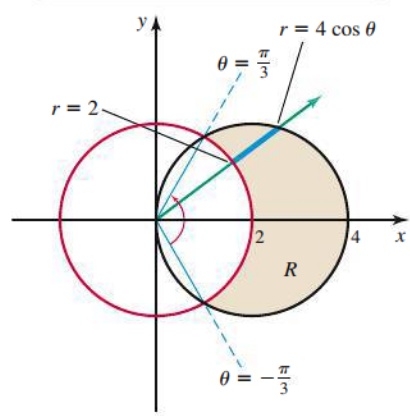
\includegraphics[width=0.35\linewidth]{images/briggs_16_03/fig16_35}
  \end{flushright}
  \pagebreak

  \begin{ex*}
    Compute the area of the region in the first and fourth quadrants outside the circle $r=\sqrt{2}$ and inside the lemniscate $r^2=4\cos(2\theta)$.
  \end{ex*}
  \begin{flushright}
    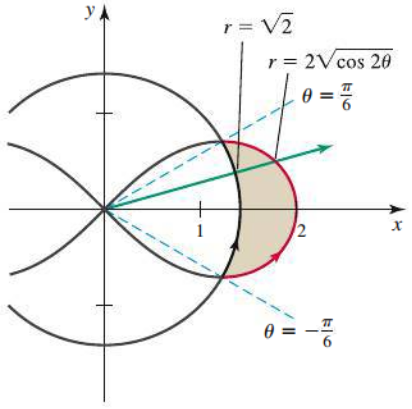
\includegraphics[width=0.35\linewidth]{images/briggs_16_03/fig16_37}
  \end{flushright}  
  \pagebreak
\end{document}
